      \documentclass[10pt]{article}  

%%%%%%%% PREÁMBULO %%%%%%%%%%%%
\title{Plantilla para prácticas de ESCOM}
\usepackage[spanish]{babel} %Indica que escribiermos en español
\usepackage[utf8]{inputenc} %Indica qué codificación se está usando ISO-8859-1(latin1)  o utf8  
\usepackage{amsmath} % Comandos extras para matemáticas (cajas para ecuaciones,
% etc)
\usepackage{amssymb} % Simbolos matematicos (por lo tanto)
\usepackage{graphicx} % Incluir imágenes en LaTeX
\usepackage{color} % Para colorear texto
\usepackage{subfigure} % subfiguras
\usepackage{float} %Podemos usar el especificador [H] en las figuras para que se
% queden donde queramos
\usepackage{capt-of} % Permite usar etiquetas fuera de elementos flotantes
% (etiquetas de figuras)
\usepackage{sidecap} % Para poner el texto de las imágenes al lado
    \sidecaptionvpos{figure}{c} % Para que el texto se alinie al centro vertical
\usepackage{caption} % Para poder quitar numeracion de figuras
\usepackage{commath} % funcionalidades extras para diferenciales, integrales,
% etc (\od, \dif, etc)
\usepackage{cancel} % para cancelar expresiones (\cancelto{0}{x})
 
\usepackage{anysize}                    % Para personalizar el ancho de  los márgenes


\marginsize{2cm}{2cm}{2cm}{2cm} % Izquierda, derecha, arriba, abajo

\usepackage{appendix}
\renewcommand{\appendixname}{Apéndices}
\renewcommand{\appendixtocname}{Apéndices}
\renewcommand{\appendixpagename}{Apéndices} 

% Para que las referencias sean hipervínculos a las figuras o ecuaciones y
% aparezcan en color
\usepackage[colorlinks=true,plainpages=true,citecolor=blue,linkcolor=blue]{hyperref}
%\usepackage{hyperref} 
%para las tablas y demás formas 
\usepackage{cdt/cdtAnalisis}
\usepackage{tikz}

% Para agregar encabezado y pie de página


\usepackage{fancyhdr} 

\pagestyle{fancy}
\fancyhf{}
\fancyhead[L]{\footnotesize ESCOM} %encabezado izquierda
\fancyhead[R]{\footnotesize IPN}   % dereecha
\fancyfoot[R]{\footnotesize Plan Ejecutivo}  % Pie derecha
\fancyfoot[C]{\thepage}  % centro
\fancyfoot[L]{\footnotesize S.E For Mobile Devices}  %izquierda
\renewcommand{\footrulewidth}{0.4pt}


\usepackage{listings} % Para usar código fuente
\definecolor{dkgreen}{rgb}{0,0.6,0} % Definimos colores para usar en el código
\definecolor{gray}{rgb}{0.5,0.5,0.5} 
% configuración para el lenguaje que queramos utilizar
\lstset{language=Matlab,
   keywords={break,case,catch,continue,else,elseif,end,for,function,
      global,if,otherwise,persistent,return,switch,try,while},
   basicstyle=\ttfamily,
   keywordstyle=\color{blue},
   commentstyle=\color{red},
   stringstyle=\color{dkgreen},
   numbers=left,
   numberstyle=\tiny\color{gray},
   stepnumber=1,
   numbersep=10pt,
   backgroundcolor=\color{white},
   tabsize=4,
   showspaces=false,
   showstringspaces=false}

\newcommand{\sen}{\operatorname{\sen}}  % Definimos el comando \sen para el seno
%en español

\title{Plantilla para trabajo terminal I de ESCOM}

%%%%%%%% TERMINA PREÁMBULO %%%%%%%%%%%%

\begin{document}

%%%%%%%%%%%%%%%%%%%%%%%%%%%%%%%%%% PORTADA %%%%%%%%%%%%%%%%%%%%%%%%%%%%%%%%%%%%%%%%%%%%
                                                                                    %%%
\begin{center}                                                                      %%%
\newcommand{\HRule}{\rule{\linewidth}{0.5mm}}                                   %%%\left
                                                                                    %%%
\begin{minipage}{0.48\textwidth} \begin{flushleft}

\includegraphics[scale = 0.1]{Imagen/ESCOM-LOGO}
\end{flushleft}\end{minipage}
\begin{minipage}{0.48\textwidth} \begin{flushright}

\includegraphics[scale = 0.35]{Imagen/IPN-LOGO}
\end{flushright}\end{minipage}

                                                                                    %%%
\vspace*{-1.5cm}                                %%%
                                                                                    %%% 
\textsc{\huge Instituto Polit\'ecnico\\ \vspace{5px} Nacional}\\[1.5cm] 

\textsc{\LARGE Escuela superior de c\'omputo}\\[1.5cm]                                                   %%%

\begin{minipage}{0.9\textwidth} 
\begin{center}                                                                                  %%%
\textsc{\LARGE Plan Ejecutivo}
\end{center}
\end{minipage}\\[0.5cm]
%%%
                                                                                    %%%
            \vspace*{1cm}                                                                       %%%
                                                                                    %%%
\HRule \\[0.4cm]                                                                    %%%
{ \huge \bfseries APP - Stay Quiet}\\[0.4cm]  %%%
                                                                                    %%%
\HRule \\[1.5cm]                                                                    %%%
                                                                                %%%
                                                                                    %%%
\begin{minipage}{0.46\textwidth}                                                    %%%
\begin{flushleft} \large                                                            %%%
\emph{Autores:}\\ 
Hernandez Soriano Gerardo  \\
Moreno Sánchez José Rodolfo\\
Perez Montiel Ulises\\
Salas Hernandez Abiran Natanael\\ 
Rincón Vieyra Alan 
%%%
            %\vspace*{2cm}  
                                                                %%%
                                                                %%%
\end{flushleft}                                                                     %%%
\end{minipage}      
                                                                %%%
\begin{minipage}{0.52\textwidth}        
\vspace{-0.6cm}                                         %%%
\begin{flushright} \large                                                           %%%
\emph{Asesor:} \\                                                                 %%%
Ulises Vélez Saldaña \\                                             %%%
\end{flushright}                                                                 %%%
\end{minipage}
\begin{figure}[htbp!]
	\begin{center}
		
\includegraphics[scale = 0.3]{Imagen/Logo_Stay_Quiet.jpg}
	\end{center}
\end{figure}                          
\begin{center}   
\vspace*{1cm}
%\begin{flushleft}
    
%\end{flushleft}
%%%
        \flushleft{\textbf{\Large S.E For Mobile Devices} }\\                                                                     %%%
\vspace{1cm}                                                                                                                              
{\large \today}                                                                 %%%
            \end{center}                                                                        
\end{center}                                                                        
                                                                                    
\newpage                                                                        
%%%%%%%%%%%%%%%%%%%% TERMINA PORTADA %%%%%%%%%%%%%%%%%%%%%%%%%%%%%%%%

\tableofcontents 

\newpage
\section{Abreviaturas.}
Se usan las siguientes abreviaturas: \\
-API		Interfaz de programación de aplicaciones \\
-BD		Base de Datos\\
-IDE		Entorno de desarrollo integrado\\ 
-GPS		Sistema de posicionamiento global\\
-RF		Requerimiento Funcional\\
-RNF		Requerimiento no Funcional\\
-SDK		Kit de desarrollo de Software\\ 
-UML		Lenguaje Unificado de Modelado 
 
\section{Introducción.}
El desarrollo de la tecnología en los últimos tiempos ha tenido grandes avances, un ejemplo de ello es en el desarrollo de dispositivos y aplicaciones móviles, los cuales tienen distintos componentes que cuantifican diversos parámetros útiles a los usuarios en su vida diaria. \\

Hasta el momento, son pocas las aplicaciones que se enfoquen en el cuidado de personas con determinadas características que requieran supervisión geográfica para su cuidado.

\newpage 
\section{Análisis del problema.}
\subsection{Contexto.}
Para reportar una persona desaparecida o extraviada se requiere esperar 72 horas. \\

Tiempo durante el cual una familia o un conjunto de personas designadas al cuidado de alguien requieren valerse de sus recursos para localizar a la persona de quien no saben donde se encuentra. \\

La señal de GPS cubre grandes áreas donde gran numero de personas habitan, por lo cual es altamente probable que se extravié un ser humano dentro de esta área   

\subsection{Planteamiento del Problema.} 
Hay seres humanos propensos a extraviarse o sufrir secuestro, por ejemplo, niños, ancianos, personas que padecen de sus facultades mentales y todos en general somos propensos a atravesar circunstancias semejantes


\subsubsection{Descomposición del problema.}
Con la intención de apoyar a las personas con determinadas necesidades de cuidar remotamente de otras, proponemos el desarrollo de un sistema para monitorio e los usuarios registrados por la persona interesada.

En el sistema se requiere identificar los siguientes módulos:
-      Módulo de registro de información personal, para que el usuario ingrese su nombre, correo electrónico, número telefónico.
-      Módulo de información geográfica, para que el usuario pueda visualizar la ubicación de sus “protegidos”.
-      Módulo de historial, para registrar los eventos relevantes y poder consultaros después.  
-      Módulo de trabajo oculto al usuario, para vigilar la actividad y advertir  al “protector” de la anomalía geográfica del “protegido”, notificándolo de forma inmediata.
-      Emplear la tecnología GPS proporcionada por el dispositivo móvil.


\subsection{Propuesta de solución.}
Desarrollar una app móvil que mediante el uso de GPS que apoye a supervisar la ubicación de una o múltiples personas dentro de un área pre establecida  
\newpage 
\subsection{Planeación del Alcance.}
\subsection{Objetivos.}
\subsubsection{General.}
Diseñar y desarrollar una aplicación móvil la cual se apoyará de los parámetros proporcionados por el GPS para supervisar la ubicación de una o múltiples personas dentro de un  área preestablecida.
\subsubsection{Específicos.}

\textbf{ Uso de GPS.} \\ 

La aplicación utiliza el servicio de GPS del celular para establecer la ubicación en un mapa  \\

\textbf{ Perfil de usuario protector.}  \\

Permite tener contactos con los cuales puede compartir su ubicación cada determinado tiempo, y se llama observador cuando se vincula a un perfil protegido \\

\textbf{ Perfil de usuario protegido.}  \\

Para las personas que se quiere cuidar, la aplicación se mantiene funcionando como GPS, se requiere introducir un password para acceder a la aplicación \\

\textbf{ Selección de área de cuidado .}  \\

El observador puede establecer una zona geografica entorno a un punto fijo en el mapa ó a una distancia de una trayectoria \\

\textbf{ Mensaje de alerta fuera de área establecida.}  \\

Si el dispositivo con el perfil protegido sale del área de cuidado el observador recibe una alerta y puede iniciar una llamada \\

\textbf{ Mensajes de alerta del dispositivo protegido .}  \\

Si el dispositivo con el perfil protegido tiene batería baja, pocos datos o señal débil, se envía un mensaje al observador
\newpage 
\subsection{Análisis de Requerimientos.}
El desarrollo del análisis de requerimientos consiste en la definición de la aplicación, se basa en los objetivos que debe cumplir, así como las funcionalidades que ha de implementar.

La información que se debe aportar de cada requerimiento es\\
\textbf{- Identificador.} Código con el que se identifica dicho requisito.\\
\textbf{- Nombre.}Nomenclatura breve y descriptiva.\\
\textbf{- Descripción.} Desarrollo de los objetivos del requisito y las condiciones que pueden limitarlo.\\
\textbf{- Dependencia.} Código de los RF que son necesarios cumplimentar para poder 
acceder a ellos.\\
\textbf{- Prioridad.} Urgencia con la que debe desarrollarse dicho requisito.\\

\subsubsection{Requerimientos Funcionales.}
Los Requerimientos Funcionales (RF) reúnen los servicios que ofrece el sistema, la reacción que debe tener en situaciones particulares y, en ciertos casos, especificará qué no debe hacer.\\

\begin{cdtRequirements}[version=1.0, author=Rodolfo, status=En espera de revisión, revisor=Ulises]
	\RFitem{RF-01}{Registrar Usuario}
	{El sistema debe registrar un perfil de usuario, con los datos personales que el usuario brinde}
	\RFitem{RF-02}{Mostrar Ubicación geográfica de protegidos}
	{El sistema debe contar con un apartado donde se muestre la ubicación geográfica de sus protegidos}
	\RFitem{RF-03}{Alerta y Notificación}
	{El sistema debe alertar al usuario mediante una notificación sobre la irregularidad en la localización o el estado de los dispositivos de sus contactos}
	\RFitem{RF-04}{Sensibilidad en monitoreo }
	{El sistema debe presentar alta sensibilidad a los cambios de ubicación de los usuarios protegidos (actualización de ubicación en periodos de tiempo cortos).}
	\RFitem{RF-05}{Actualización de ubicación geográfica}
	{El sistema debe actualizar los datos de la ubicación de los protegidos en la aplicación móvil del protector; en un intervalos menores de 1 minuto para el estado de reposo, y menor de 5 segundos cuando el estado es de alerta.}
	\RFitem{RF-06}{Alerta de riesgos}
	{El sistema debe notificar al usuario si surgen imprevistos, (batería baja, pocos datos móviles disponibles o señal deficiente)}
	\RFitem{RF-07}{Comunicación con protegido}
	{El sistema proporciona comunicación entre los usuarios, ésta puede ser llamada telefónica y/o mensajes}
	\RFitem{RF-08}{Rango de protección}
	{El sistema brinda al protector la opción de definir un rango o una zona preestablecida de protección para sus protegidos}
	\RFitem{RF-09}{Agregar protegidos}
	{El sistema brinda al protector  la opción de  agregar n número de protegidos a su cuenta.}
	\RFitem{RF-10}{El usuario protector  podrá agregar n número de protegidos a su cuenta.}
	{El sistema debe implementar un sistema de control de acceso a los usuarios que tengan el rol de protegido, vía pin y correo electrónico  proporcionados por el protector.}
	
	
\end{cdtRequirements}
\newpage 
\subsubsection{Requerimientos No Funcionales.}
Los Requerimientos No Funcionales (RNF) no hacen referencia a funciones del sistema, describen propiedades que éste debe cumplir. De este modo, se restringe de forma indirecta la aplicación.\\


\begin{cdtRequirementsNF}[version=1.0, author=Rodolfo, status=En espera de aprobación del asesor, revisor=Ulises]
	\RFitem{RNF-01}{Política de privacidad}
	{Al termino del registro del usuario en el sistema, se le deberá presentar la Política de Privacidad, la cual le explicará que sus datos serán confidenciales..}
	\RFitem{RNF-02}{Disponibilidad del Sistema}
	{El sistema deberá estar disponible cuando el usuario así lo requiera.}
	\RFitem{RNF-03}{Documentación del sistema}
	{El sistema deberá disponer de una documentación actualizable que permita realizar las operaciones de mantenimiento con la mayor eficacia posible.}
	\RFitem{RNF-04}{Almacenamiento de Información}
	{El sistema deberá almacenar la información del usuario en el almacenamiento local del teléfono inteligente.}
	\RFitem{RNF-05}{Copia de Seguridad}
	{El sistema deberá ser integrado a la API de copia de seguridad automática del sistema operativo nativo del teléfono inteligente.}
\end{cdtRequirementsNF}

\newpage 
\section{Planeación de tiempo}

\subsection{Metodología}
La IEEE define la ingeniería de software como la aplicación de un enfoque sistemático, disciplinado y cuantificable al desarrollo, operación y mantenimiento del software; es decir, la aplicación de ingeniería al software.\\ 

La ingeniería de se fundamenta en el compromiso con la calidad.\\

Para el óptimo desarrollo de este proyecto se acordó aplicar Ingeniería de Software, con base en la metodología de desarrollo para móviles, Mobile-D.\\

Esta técnica consiste en la creación de software dividida en cuatro etapas fundamentales:\\

\textbf{1. Análisis de requerimientos:} Se determinan los requisitos que debe de cumplimentar el software. Esta etapa es crucial para llegar a lograr los objetivos finales.\\

\textbf{2. Diseño y arquitectura:} Se establece un diseño conceptual de la aplicación a través de los Casos de Uso. Se muestran también en este apartado los primeros mockups de la aplicación.\\

\textbf{3. Desarrollo e implementación:} Se traslada el diseño realizado en el paso anterior a código. Se percibirán los primeros resultados de la aplicación en funcionamiento.\\

\textbf{4. Pruebas:} Es la fase final. Se comprueba el correcto funcionamiento de la aplicación.

\subsubsection{Mobile-D}

Esta metodología está basada en diversas tecnologías como Rational UnifiedProcess, Extreme Programming y Crystal Mehodologies, y su finalidad es intentar obtener pequeños ciclos de desarrollo de forma rápida en dispositivos pequeños. \\

Un ciclo de proyecto con la metodología Mobile-D está compuesto por cinco fases:\\

\textbf{Fase de Exploración}\\

Esta fase es la encargada de la planificación y educción de requisitos del proyecto, donde tendremos la visión completa del alcance del proyecto y también todas las funcionalidades del producto.  \\

\textbf{Fase de inicialización}\\

La fase de inicialización es la implicada en conseguir el éxito en las próximas fases del proyecto, donde se preparará y verificará todo el desarrollo y todos los recursos que se necesitarían. Esta fase se divide en cuatro etapas: la puesta en marcha del proyecto, la planificación inicial, el día de prueba y día de salida.\\

\textbf{Fase de producción}\\

En la fase de producción, se vuelve a repetir la programación de los tres días, iterativamente hasta montar (implementar) las funcionalidades que se desean. Aquí usamos el desarrollo dirigido por pruebas (TDD), para verificar el correcto funcionamiento de los desarrollos. \\

\textbf{Fase de estabilización} \\

Se llevarán a cabo las últimas acciones de integración donde se verificará el completo funcionamiento del sistema en conjunto. De toda la metodología, esta es la fase más importante de todas ya que es la que nos asegura la estabilización del desarrollo. También se puede incluir en esta fase, toda la producción de documentación. \\

\textbf{Fase de pruebas} \\

Es la fase encargada del testeo de la aplicación una vez terminada. Se deben realizar todas las pruebas necesarias para tener una versión estable y final. En esta fase, si nos encontramos con algún tipo de error, se debe proceder a su arreglo pero nunca se han de realizar desarrollos nuevos de última hora, ya que nos haría romper todo el ciclo. [A] \\
\newpage 

\subsubsection{Cronograma}
\begin{figure}[htbp!]
	\begin{center}
		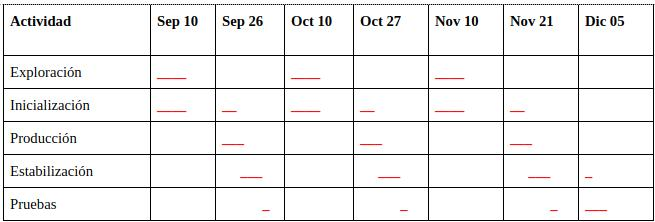
\includegraphics[scale = 0.6]{Imagen/Cronograma.jpg}
	\end{center}
\end{figure}

\newpage 

\subsection{Roles:}
\section{Planeación de Recursos Humanos:}

\subsection{Roles:}
\begin{figure}[htbp!]
	\begin{center}
		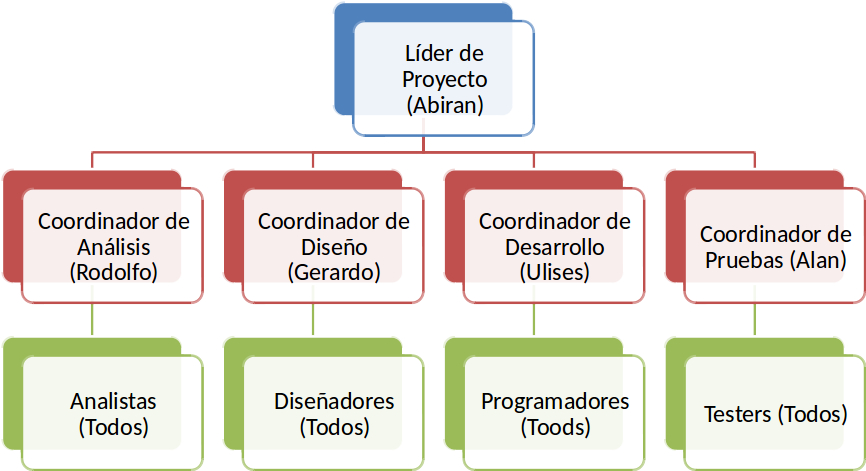
\includegraphics[scale = 0.5]{Imagen/organigrama.jpg}
	\end{center}
\end{figure}
\newpage 
\subsection{Responsabilidades.}


\textbf{Líder de proyecto}
\begin{itemize}
 \item Reconocer los riesgos que puedan impactar la probabilidad de éxito del proyecto.
 \item Crear políticas para reducir el impacto de los riesgos.
 \item Planear la ejecución del proyecto en su totalidad.
 \item Resolver los problemas que se presenten durante la ejecución del proyecto.
 \item Crear acuerdos entre los coordinadores de las áreas involucradas en el proyecto.\\
\end{itemize}

\textbf{Coordinador de Análisis}
\begin{itemize}
 \item Establecer la forma de trabajo de los analistas y darla a conocer a todo el equipo.
 \item Asignar tareas a los miembros del equipo de análisis.
 \item Registrar los tiempos requeridos para realizar las tareas de análisis.
 \item Realizar el mapeo de procesos.
 \item Documentar requerimientos.
 \item Documentar casos de uso.
 \item Identificar y documentar reglas y términos de negocio.
 \item Diseñar pantallas.
 \item Realizar mapas de navegación.
 \item Responder las dudas en torno al análisis.
 \item Supervisar el avance del equipo de análisis.
 \item Establecer acuerdos con el resto de los coordinadores.
 \item Verificar el trabajo de los analistas.
 \item Participar en las reuniones de mejora de procesos.
 \item Documentar lecciones aprendidas.\\
\end{itemize}
\newpage 
\textbf{Analista}
\begin{itemize}
 \item Realizar el mapeo de procesos.
 \item Documentar requerimientos.
 \item Documentar casos de uso.
 \item Identificar y documentar reglas y términos de negocio.
 \item Diseñar pantallas.
 \item Realizar mapas de navegación.
 \item Notificar avance al Coordinador de Análisis.
 \item Notificar cualquier cambio al alcance al Coordinador de Análisis.
 \item Documentar lecciones aprendidas.
 \item Participar en las reuniones de mejoras de procesos.\\
\end{itemize}

\textbf{Coordinador de Diseño}
\begin{itemize}
 \item Establecer la forma de trabajo de los diseñadores y darla a conocer a todo el equipo.
 \item Planear las actividades de la etapa de diseño.
 \item Asignar tareas a los miembros del equipo de diseño.
 \item Traducir los elementos de análisis a en clases y entidades.
 \item Realizar los diagramas de secuencia para los procesos del sistema.
 \item Generar el diagrama entidad-relación de la base de datos.
 \item Responder las dudas en torno al diseño del sistema.
 \item Supervisar el avance del equipo de diseño.
 \item Establecer acuerdos con el resto de los coordinadores.
 \item Verificar el trabajo de los diseñadores.
 \item Apoyar al arquitecto de software en la definición de la infraestructura.
 \item Participar en las reuniones de mejora de procesos.
 \item Registrar los tiempos requeridos para realizar las tareas de diseño.
 \item Documentar lecciones aprendidas.\\
\end{itemize}
\newpage 
\textbf{Diseñador}
\begin{itemize}
 \item Traducir los elementos de análisis en clases y entidades.
 \item Generar el diagrama entidad-relación de la base de datos.
 \item Realizar los diagramas de secuencia para los procesos del sistema.
 \item Informar al Coordinador de Diseño sobre posibles cambios o problemas en la arquitectura del sistema.
 \item Notificar al Coordinador de Diseño el avance.
 \item Participar en las reuniones de mejoras de procesos.
 \item Documentar lecciones aprendidas.\\
\end{itemize}

\textbf{Coordinador de Desarrollo}
\begin{itemize}
 \item Establecer la forma de trabajo de los programadores y darla a conocer a todo el equipo.
 \item Planear las actividades de la etapa de implementación.
 \item Asignar tareas a los miembros del equipo de desarrollo.
 \item Implementar los componentes necesarios para los casos de uso asignados, definidos en el diseño.
 \item Realizar pruebas funcionales sobre los elementos programados.
 \item Enrolar buenas prácticas de programación para el proyecto.
 \item Asegurar la integración de los módulos del sistema.
 \item Responder las dudas en torno a la programación del sistema.
 \item Supervisar el avance del equipo de desarrollo.
 \item Establecer acuerdos con el resto de los coordinadores.
 \item Verificar el trabajo de los programadores.
 \item Apoyar al arquitecto de software (Coordinador de diseño) en la definición de la infraestructura.
 \item Participar en las reuniones de mejora de procesos.
 \item Definir la forma de solucionar las incidencias reportadas en la programación.
 \item Registrar los tiempos requeridos para realizar las tareas de desarrollo.
 \item Documentar lecciones aprendidas.\\
\end{itemize}
\newpage 
\textbf{Programador}
\begin{itemize}
 \item Implementar los componentes necesarios para los casos de uso asignados, definidos en el diseño.
 \item Realizar pruebas funcionales sobre los elementos programados.
 \item Aplicar las buenas prácticas de programación definidas para el proyecto.
 \item Asegurar la integración de los módulos del sistema.
 \item Notificar el avance al Coordinador de Programación.
 \item Participar en las reuniones de mejoras de procesos.
 \item Documentar lecciones aprendidas.\\
\end{itemize}

\textbf{Coordinador de Pruebas}
\begin{itemize}
 \item Establecer la forma de trabajo de los testers y darla a conocer a todo el equipo.
 \item Planear las actividades de la etapa de pruebas.
 \item Asignar tareas a los miembros del equipo de pruebas.
 \item Identificar los escenarios a probar en un caso de uso, módulo o sistema.
 \item Documentar los guiones de prueba del sistema.
 \item Documentar los datos de prueba.
 \item Ejecutar las pruebas y documentar los resultados.
 \item Dar retroalimentación a los programadores sobre los resultados.
 \item Dar seguimiento a las incidencias encontradas.
 \item Responder las dudas en torno a las pruebas e incidencias encontradas dentro del sistema.
 \item Supervisar el avance del equipo de pruebas.
 \item Supervisar que el proceso de pruebas se realice correctamente.
 \item Establecer acuerdos con el resto de los coordinadores.
 \item Verificar el trabajo de los testers.
 \item Participar en las reuniones de mejora de procesos.
 \item Registrar los tiempos requeridos para realizar las tareas de pruebas.
 \item Documentar lecciones aprendidas.\\
\end{itemize}
\newpage 
\textbf{Tester}
\begin{itemize}
 \item Identificar los escenarios a probar en un caso de uso, módulo o sistema.
 \item Documentar los guiones de prueba del sistema.
 \item Documentar los datos de prueba.
 \item Generar los scripts de prueba para cada escenario.
 \item Ejecutar las pruebas y documentar los resultados.
 \item Dar retroalimentación a los programadores sobre los resultados.
 \item Dar seguimiento a las incidencias encontradas.
 \item Notificar el avance al Coordinador de Pruebas.
 \item Notificar al Coordinador de Pruebas de posibles fallos en el análisis o implementación.
 \item Participar en las reuniones de mejoras de procesos.
 \item Documentar lecciones aprendidas.\\
\end{itemize}

\subsection{Contacto.}

\textbf{Hernández Soriano Gerardo}\\
Alumno de la carrera de Ingeniería en Sistemas Computacionales en ESCOM\\
Tel. 55 2974 7782\\
Correo electrónico: ghernandezs1609@gmail.com\\

\textbf{Moreno Sánchez José Rodolfo} \\
Alumno de la carrera de Ingeniería en Sistemas Computacionales en ESCOM\\
Tel. 55 2801 2620 \\
Correo electrónico: rodmorz@gmail.com \\

\textbf{Pérez Montiel Ulises} \\
Alumno de la carrera de Ingeniería en Sistemas Computacionales en ESCOM\\
Tel. 55 1617 9751 \\
Correo electrónico: uperezm1001@gmail.com\\

\textbf{Salas Hernández Abiran Natanael}\\
Alumno de la carrera de Ingeniería en Sistemas Computacionales en ESCOM\\
Tel. 55 7275 3650\\
Correo electrónico: abisaher@gmail.com\\

\textbf{Rincón Vieyra Alan}\\
Alumno de la carrera de Ingeniería en Sistemas Computacionales en ESCOM\\
Tel. 55 4062 3689\\
Correo electrónico: alanVieyra376@gmail.com

\section{Referencias.}
\textbf{[A] Metodología Mobile-D. 2015. Disponible en:}\\ http://manuelguerrero.blogspot.es/1446543763/metodologia-mobile-d-para-desarrollos-de-aplicaciones-moviles/
\end{document}